% ============================================================
%  part3/ch13-phase-transitions.tex
%  Chapter 13: Phase Transitions
% ============================================================

\chapter{Phase Transitions}
\label{ch:phase-transitions}

\epigraph{%
  How does symmetry become structure?%
}{---}

\begin{WhyChapter}
  The Ising model (Chapter~\ref{ch:ising}) showed that two
  ground states exist.
  This chapter asks the prior question: why does a system
  ever leave the symmetric, disordered phase?
  The answer --- Landau theory, bifurcation, and critical
  phenomena --- provides the mathematical language for every
  subsequent coarsening discussion.
  Without understanding phase transitions, the appearance of
  domains, filaments, and voids would be mysterious.
  With it, they become inevitable.
\end{WhyChapter}


\begin{ChapterIntro}
There are moments when a system changes not because something new was added, but because something already present becomes organised. Water freezes. A magnet aligns. A crowd begins moving in the same direction. Nothing fundamentally new has appeared. The components are the same. What changes is the pattern of relationships among them.

From far away, such transitions can seem abrupt. Up close, they emerge from countless local interactions, each responding only to its immediate surroundings. The remarkable fact is that large-scale order often arises without any central coordinator.

The mathematics of phase transitions exists to describe how local interactions become global structure. Before we can understand how cosmic structure forms, we must understand how order emerges in simpler settings.
\end{ChapterIntro}

\section{Order parameters and macrostates}

The central object is the \emph{order parameter}: a quantity
that is zero in the disordered phase and nonzero in the
ordered phase.

\begin{definition}[Order parameter]
  \label{def:order-param}
  For an Ising system of $N$ spins,
  \[
    m = \frac{1}{N}\sum_i \sigma_i \in [-1,+1].
  \]
  More generally, an order parameter is any scalar, vector,
  or tensor field that vanishes in the high-symmetry phase.
\end{definition}

\begin{example}[Order parameters across systems]
  Ising magnet: $m$ (magnetisation).
  Liquid crystal: $Q_{ij}$ (alignment tensor).
  Superfluid: $\psi \in \mathbb{C}$ (condensate amplitude).
  RSVP: $\Phi$ (scalar plenum density).
\end{example}

\section{Landau theory}

\begin{definition}[Landau free energy]
  \label{def:landau}
  Near a continuous phase transition,
  \[
    F(m) = a(T - T_c)m^2 + bm^4, \quad b > 0.
  \]
\end{definition}

\begin{theorem}[Emergence of ordered states]
  \label{thm:phase-emergence}
  \statusproven{}
  For $T > T_c$, the unique minimum is $m = 0$.
  For $T < T_c$, two nontrivial minima emerge:
  \[
    m_\pm = \pm\sqrt{\frac{a(T_c - T)}{2b}}.
  \]
\end{theorem}

\begin{proof}
  Critical points: $\frac{dF}{dm} = 2a(T-T_c)m + 4bm^3 = 0$,
  so $m(a(T-T_c) + 2bm^2) = 0$.
  Hence $m = 0$ or $m^2 = a(T_c-T)/(2b)$.
  For $T > T_c$: $a(T-T_c) > 0$, so $m^2 < 0$ has no real
  solution; $m=0$ is a minimum.
  For $T < T_c$: $m^2 = a(T_c-T)/(2b) > 0$, giving $m_\pm$.
  Second derivative confirms $m=0$ is a maximum and $m_\pm$
  are minima.
\end{proof}

\begin{TechNote}[Phase transitions create structure without new forces]
  A phase transition is not the appearance of a new force.
  It is the appearance of new minima.
  The same Hamiltonian that had one ground state now has two.
  Structure appears because the symmetric state becomes unstable,
  not because something new acts on the system.
  This sentence is crucial for RSVP: cosmic structure need not
  require new forces if the plenum field undergoes a
  phase-ordering transition.
\end{TechNote}

\section{Bifurcation structure}

The transition at $T_c$ is a \emph{pitchfork bifurcation}.

\begin{proposition}[Bifurcation from symmetric phase]
  \label{prop:pitchfork}
  \statusproven{}
  As $T$ decreases through $T_c$, the solution branch
  $m = 0$ loses stability and two stable branches
  $m = \pm m_\star(T)$ emerge, where
  $m_\star(T) \sim (T_c - T)^{1/2}$ near $T_c$.
\end{proposition}

\begin{proof}
  Stability: $F''(0) = 2a(T-T_c)$.
  For $T > T_c$: $F''(0) > 0$, $m=0$ stable.
  For $T < T_c$: $F''(0) < 0$, $m=0$ unstable.
  The emerging branches have $F''(m_\pm) = -4a(T-T_c) > 0$,
  confirming stability.
  $m_\star = \sqrt{a(T_c-T)/(2b)} \sim (T_c-T)^{1/2}$.
\end{proof}

\begin{definition}[Critical exponent $\beta$]
  The order parameter vanishes as
  $m_\star \sim (T_c - T)^\beta$ near $T_c$.
  For Landau theory: $\beta = 1/2$.
\end{definition}

\section{Fluctuations and the Ginzburg criterion}

Mean-field theory ignores fluctuations.
The Ginzburg criterion determines when this is valid.

\begin{definition}[Ginzburg--Landau functional]
  \[
    \mathcal{F}[\phi]
    = \int\left[\tfrac{1}{2}r\phi^2 + \tfrac{1}{4}u\phi^4
      + \tfrac{1}{2}|\nabla\phi|^2\right]dx,
    \quad r = a(T - T_c).
  \]
\end{definition}

\begin{theorem}[Ginzburg criterion]
  \label{thm:ginzburg}
  \statusproven{}
  Mean-field theory is valid iff
  $\langle(\delta\phi)^2\rangle / \phi_0^2 \ll 1$.
  For $d < 4$, this fails near $T_c$: mean-field breaks down.
\end{theorem}

\begin{proof}
  Gaussian fluctuation variance:
  $\langle(\delta\phi)^2\rangle
  = \int \frac{d^dk}{(2\pi)^d}\frac{1}{k^2+r}
  \sim \xi^{4-d}$ as $r \to 0$,
  where $\xi = r^{-1/2}$ is the correlation length.
  The order parameter satisfies $\phi_0^2 \sim |r|/u$.
  Therefore $\langle(\delta\phi)^2\rangle/\phi_0^2
  \sim u\xi^{4-d} \to \infty$ as $\xi \to \infty$ for $d < 4$.
  Mean-field fails below the upper critical dimension $d_c = 4$.
\end{proof}

\begin{TechNote}[Upper critical dimension]
  For $d < 4$ (including $d = 3$, the physical universe),
  fluctuations are important near $T_c$.
  The critical exponents differ from mean-field values.
  This is the origin of universality classes: systems with
  different microscopic physics but the same symmetry, dimension,
  and conservation laws share the same critical exponents.
\end{TechNote}

\section{Critical slowing down}

\begin{theorem}[Critical slowing down]
  \label{thm:critical-slow}
  \statusproven{}
  Near $T_c$, the relaxation time diverges:
  $\tau \sim \xi^z$,
  where $z$ is the dynamic exponent.
\end{theorem}

\begin{proof}
  Linearise $\partial_t\phi = -r\phi + \Delta\phi$ around $\phi = 0$.
  Fourier modes satisfy
  $\partial_t\hat\phi_k = -(r + k^2)\hat\phi_k$.
  Relaxation time: $\tau_k = 1/(r+k^2)$.
  For the slowest mode $k \to 0$: $\tau \sim 1/r \sim \xi^2$
  (with $z = 2$ for this equation).
  More generally, different dynamics give different $z$.
\end{proof}

\begin{ForwardRef}
  Critical slowing down anticipates the coarsening dynamics
  of Chapter~\ref{ch:allen-cahn}: near the transition, the
  system evolves very slowly because the restoring force
  vanishes.
  The dynamic exponent $z$ introduced here is the same $z$
  in the coarsening law $\ell(t) \sim t^{1/z}$.
\end{ForwardRef}

\begin{ChapterConnection}
  This chapter established: symmetry breaking gives two
  ground states; Landau theory describes the bifurcation;
  Ginzburg criterion shows when fluctuations matter;
  critical slowing introduces $z$.
  Chapter~\ref{ch:domain-formation} now asks: once two
  phases coexist, how does spatial structure evolve?
\end{ChapterConnection}

\begin{ProblemSet}
\problem{
  For the Landau free energy $F(m) = a(T-T_c)m^2 + bm^4$
  with $a = 1$, $b = 1$, $T_c = 1$:
  (a) Find $m_\pm$ at $T = 0$.
  (b) Compute $F(m_\pm)$ and compare to $F(0)$.
  (c) Sketch $F(m)$ for $T = 0$, $T = T_c$, $T = 2T_c$.
}
\problem{
  Show that the bifurcation in Theorem~\ref{prop:pitchfork}
  is a \emph{supercritical} pitchfork: the emerging branches
  $m_\pm$ are stable and the transition is continuous.
  What would a \emph{subcritical} bifurcation look like,
  and what physical phenomenon would it describe?
}
\problem{
  For the Ginzburg--Landau functional, compute the
  susceptibility $\chi = d\langle\phi\rangle/dh$ where $h$ is
  an external field added as $-h\phi$.
  Show that $\chi$ diverges as $T \to T_c$.
}
\problem{
  \textbf{Reconstruction exercise.}
  Suppose you observe $m = 0.3$ in an Ising system.
  Can you determine whether the system is above or below $T_c$?
  What additional observations would allow you to determine
  the temperature? What information is irretrievably lost?
}
\end{ProblemSet}

\section{Susceptibility divergence}

\begin{proposition}[Susceptibility divergence at $T_c$]
  \label{prop:susceptibility}
  \statusproven{}
  In an external field $h$, the susceptibility
  $\chi = \partial m/\partial h$ satisfies
  \[
    \chi \approx \frac{1}{2a(T-T_c)} \to \infty
    \quad\text{as}\quad T \to T_c^+.
  \]
\end{proposition}

\begin{proof}
  Add $-hm$ to the Landau free energy:
  $F(m) = a(T-T_c)m^2 + bm^4 - hm$.
  Equilibrium: $2a(T-T_c)m + 4bm^3 = h$.
  For $T > T_c$ and small $h$: $m$ is small, cubic term negligible,
  so $m \approx h/[2a(T-T_c)]$.
  Differentiating: $\chi = \partial m/\partial h
  \approx 1/[2a(T-T_c)] \to \infty$ as $T \to T_c^+$.
\end{proof}

\begin{TechNote}[What susceptibility divergence means]
  At $T_c$, the system becomes globally sensitive to infinitesimal
  external influences.
  A tiny field $h$ can align the entire system.
  This is the first concrete example of a phenomenon where local
  interactions produce global sensitivity --- a theme that
  reappears in RSVP as the lamphron stabilisation/lamphrodyne
  relaxation balance near critical coarsening regimes.
\end{TechNote}

% ---- Figures ------------------------------------------------

\begin{figure}[ht]
\centering
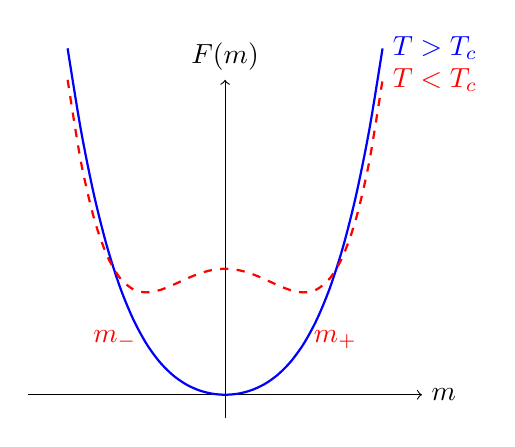
\begin{tikzpicture}[scale=1.0]
  \draw[->] (-2.5,0) -- (2.5,0) node[right] {$m$};
  \draw[->] (0,-0.3) -- (0,4) node[above] {$F(m)$};
  % T > Tc: single minimum
  \draw[domain=-2:2,smooth,thick,blue]
    plot (\x,{0.5*(\x)^2 + 0.15*(\x)^4})
    node[right,blue] {$T>T_c$};
  % T < Tc: double well
  \draw[domain=-2:2,smooth,thick,red,dashed]
    plot (\x,{-0.6*(\x)^2 + 0.3*(\x)^4 + 1.6})
    node[right,red] {$T<T_c$};
  \node at (-1.4,0.7) [red] {$m_-$};
  \node at ( 1.4,0.7) [red] {$m_+$};
\end{tikzpicture}
\caption{Landau free energy above and below $T_c$.
         For $T>T_c$ (solid, blue) the unique minimum is $m=0$.
         For $T<T_c$ (dashed, red) two minima $m_\pm$ emerge,
         spontaneously breaking the $m\mapsto -m$ symmetry.}
\label{fig:landau-well}
\end{figure}

\begin{figure}[ht]
\centering
\begin{tikzpicture}
  \draw[->] (-0.3,0) -- (4.5,0) node[right] {$T$};
  \draw[->] (0,-2.2) -- (0,2.2) node[above] {$m$};
  \draw[very thick] (0,0) -- (2,0);          % stable m=0 for T>Tc
  \draw[very thick,blue]                      % upper branch
    plot[domain=2:4.4,smooth] (\x,{sqrt(\x-2)});
  \draw[very thick,blue]                      % lower branch
    plot[domain=2:4.4,smooth] (\x,{-sqrt(\x-2)});
  \node at (2,-0.25) {$T_c$};
  \draw[dashed] (2,0) -- (2,-0.2);
\end{tikzpicture}
\caption{Pitchfork bifurcation at $T_c$.
         The symmetric branch $m=0$ is stable for $T>T_c$ (heavy line)
         and unstable below it, where two stable branches $m_\pm$
         bifurcate.}
\label{fig:pitchfork}
\end{figure}

\begin{CitationAnchor}
  The Landau free-energy expansion~\eqref{def:landau} follows the
  phenomenological framework introduced by Landau (1937).
  The pitchfork bifurcation structure is a standard result in
  the theory of symmetry breaking; see Goldenfeld~\cite{goldenfeld1992}
  for a modern pedagogical treatment.
  The Ginzburg criterion (Theorem~\ref{thm:ginzburg}) and the
  resulting upper critical dimension $d_c = 4$ are discussed
  in detail in Wilson's renormalisation-group programme
  (Wilson \& Kogut 1974).
\end{CitationAnchor}

\begin{FurtherReading}
  The standard graduate introduction to phase transitions and
  critical phenomena is Goldenfeld's \textit{Lectures on Phase
  Transitions and the Renormalization Group} (1992).
  For a more mathematical treatment of Landau theory and
  bifurcation, see Chaikin \& Lubensky~\cite{chaikin1995}.
  Renormalisation-group methods and universality classes are
  developed in Wilson \& Kogut (1974) and the monograph by
  Cardy (1996).
\end{FurtherReading}
